\section{Experiments}\label{sec:experiments}

\subsection{Experimental Setup}
\label{subsec:41}

\textbf{Datasets and metrics.} We use K-Radar as the primary benchmark and extend the evaluation to V2X-Radar-V to examine the architecture under different sensor inputs and object categories \citep{paek2022kradar,yang2025v2xradar}. K-Radar v1 evaluates Sedan within a region of \([0,72]\times[-6.4,6.4]\times[-2,6]\) m, with 10,065 test frames after filtering. Version v2 uses revised labels, expands the lateral and vertical ranges to \([-16,16]\) and \([-2,7.6]\) m, and evaluates Sedan and Bus/Truck over 13,727 test frames. We report 3D and bird's-eye-view average precision, denoted by \(\mathrm{AP}_{3D}\) and \(\mathrm{AP}_{BEV}\); Mean on v2 is the arithmetic mean over the two classes. Main K-Radar results use a confidence prefilter of 0.3. Additional thresholds, complete IoU results, and the evaluator differences between v1 and v2 are detailed in Appendices~\ref{app:b} and~\ref{app:c}. On V2X, we use deduplicated validation and test sets containing 1,487 and 1,486 frames. We report Moderate AP\(_{R40}\) at IoU thresholds of 0.7, 0.5, and 0.5 for Vehicle, Pedestrian, and Cyclist, respectively.

\textbf{Compared methods and model configurations.} We distinguish published results, results associated with released checkpoints, and local training runs. The v1 experiments use the complete ObjDec architecture described in Section~\ref{sec:methods}. For v2, we evaluate DecControlled Strong, which retains shared and modality-specific representations, foreground gating, and modality contribution control, but omits object context and its query/output modulation. This setting examines decoupled control under wider spatial coverage and an additional category. ASF serves as the direct three-sensor fusion reference, while L4DR provides a LiDAR--radar architectural comparison \citep{paek2025asf,huang2025l4dr}. The V2X ASF-style baseline retains unified projection, local attention, and subsequent feature transformation, with the ObjDec representation branches and control paths removed from the common backbone; this adaptation does not use SCL. Sources, modalities, and initialization differences are identified in the tables or captions.

\textbf{Training and model selection.} The K-Radar ASF/ObjDec models use pretrained modality encoders with frozen parameters, while BatchNorm statistics follow the original training behavior. We use AdamW~\citep{loshchilov2019adamw} for training. Local v2 comparisons use the same training set, 11 epochs, and an effective batch size of 2, followed by evaluation of the final checkpoint. ASF and Strong use the same pretrained encoders, whereas L4DR trains its native network from scratch; this comparison therefore matches the training schedule and sample budget. The full v1 model and ablated variants undergo preliminary evaluation on 1,000 samples for checkpoint selection, followed by full-set evaluation; Appendix~\ref{app:b} documents the available selection procedure and the provenance details still to be completed. V2X uses an 80-epoch budget and an effective batch size of 8, selecting checkpoints by validation mean \(\mathrm{AP}_{3D}\) before testing. ASF's sensor-combination supervision is retained in the primary K-Radar configurations and disabled in the V2X adaptation. Network dimensions, learning-rate schedules, and loss weights are provided in Appendix~\ref{app:a}.

\subsection{Detection Performance on K-Radar}
\label{subsec:42}

\textbf{Main results on v1.} Table~\ref{tab:1} compares methods under the Sedan narrow-region setting. ObjDec achieves 88.36 \(\mathrm{AP}_{3D}@0.3\) and 88.10 \(\mathrm{AP}_{BEV}@0.5\), improving over the results associated with the released ASF checkpoint at the same confidence threshold by 8.04 and 7.77 percentage points. At the stricter \(\mathrm{AP}_{3D}@0.5\), performance increases from 67.19 to 67.50. The gains in this comparison are concentrated at the lower 3D IoU threshold and in BEV detection. We also report a locally retrained ASF reference: ObjDec improves \(\mathrm{AP}_{BEV}@0.5\) by 7.73 points, achieves similar \(\mathrm{AP}_{3D}@0.5\), and is 0.22 points lower in \(\mathrm{AP}_{3D}@0.3\). Appendix~\ref{app:c} reports confidence sensitivity; with the additional confidence filter set to 0.0, ObjDec and the same official ASF archive achieve 88.06 and 87.34 \(\mathrm{AP}_{3D}@0.3\). The reported gains are therefore specific to the checkpoints and evaluation settings shown.

\textbf{Extended setting on v2.} Table~\ref{tab:2} evaluates wider spatial coverage and two object categories. Under the matched training schedule, DecControlled Strong achieves mean \(\mathrm{AP}_{3D}@0.3/@0.5/@0.7\) of 66.91/43.05/11.11, exceeding locally trained ASF by 2.14/3.36/1.56 percentage points. All six aggregate 3D/BEV metrics in the complete results improve numerically. Bus/Truck \(\mathrm{AP}_{3D}@0.5\) increases from 27.88 to 33.97, showing gains on a category beyond the primary v1 setting. Strong also exceeds the official ASF archive by 1.48 points in mean \(\mathrm{AP}_{3D}@0.5\). The released L4DR checkpoint remains stronger in mean \(\mathrm{AP}_{3D}@0.3/@0.5\), reflecting differences in architecture and training conditions. These results support the applicability of the decoupled-control variant to the extended setting.

\textbf{Conditions and sensor availability.} Appendices~\ref{app:c} and~\ref{app:f} report weather breakdowns and missing/corrupted-input analyses with fixed model weights. On v2, Strong improves over locally trained ASF in 24 of the 26 valid weather--class entries at IoU 0.3 and 0.5, with decreases in the remaining two entries. On v1, removing the camera yields 88.06 \(\mathrm{AP}_{3D}@0.3\), close to 88.36 with all sensors, whereas removing LiDAR reduces it to 57.62. The model thus retains performance under some input changes while remaining dependent on LiDAR. We treat weather groups and sensor availability as conditional analyses and report the complete combinations and exceptions in the appendix.

\subsection{Component Ablations and Computational Cost}
\label{subsec:43}

\textbf{Representation supervision and fusion control.} Table~\ref{tab:3} examines the constraints used to learn the decoupled representations and the mechanisms through which they guide fusion. Removing decoupling supervision retains the shared and modality-specific branches and all forward control paths, but reduces \(\mathrm{AP}_{3D}@0.3/@0.5\) from 88.36/67.50 to 80.23/66.16. This comparison supports the contribution of the representation constraints within the proposed architecture. Fixing the foreground gate to one and removing its supervision yields 80.00/64.80, indicating the value of learned spatial modulation. Disabling modality contribution control produces 79.62/64.38, while removing object context yields 80.14/66.23. Under the reported selection and evaluation procedure, all four changes reduce both metrics, supporting the joint learning and use of decoupled representations for detection. Appendix~\ref{app:d} provides stricter 3D and additional BEV metrics omitted here, together with implementation details of each ablation.

\textbf{Computational cost.} ObjDec increases the parameter count from 78.13M to 79.47M relative to ASF, an increase of approximately 1.7\%. In paired measurements on an RTX A6000 with batch size 1, standard eager execution takes 84.00 ms for ASF and 84.69 ms for ObjDec. Timing includes preprocessing, device transfer, encoding, fusion, detection decoding, and NMS, while excluding disk loading and collation. With the same CUDA Graph optimization, the times are 59.30 and 59.57 ms, respectively, indicating a small latency overhead for the added computation paths. The optimized path has undergone sampled numerical checks but has not yet been evaluated for full-test AP; Appendix~\ref{app:h} separately documents its timing protocol, numerical checks, and runtime limitations.

\subsection{Representation and Qualitative Analysis}
\label{subsec:44}

\textbf{Shared and modality-specific representations.} We analyze all 10,065 v1 test frames, covering 51 sequences and 642,649 foreground patch locations. Figure~\ref{fig:3} shows input, shared, and modality-specific representations under normal and heavy-snow conditions. Each point represents the mean feature over one frame's GT-defined foreground patches; the PCA bases are fitted using all weather groups. Shared and modality-specific branches exhibit different distribution structures, with residual modality-related structure also visible in shared features. Separately, cosine similarity is computed at matched foreground locations in the original 256-dimensional space and averaged within frames and weather groups. Across seven weather groups, mean cross-modal cosine ranges from 0.951 to 0.959 for shared representations and from 0.446 to 0.549 for modality-specific representations. These statistics describe feature organization rather than establish semantic identifiability: frame-level mismatch controls also yield high shared cosine before centering. We therefore interpret the visualizations alongside the representation-supervision ablation in Table~\ref{tab:3}. Appendix~\ref{app:e} provides all-weather PCA, original-space distributions, and correspondence controls.

\textbf{Spatial gating and detection.} Figure~\ref{fig:4} relates predicted foreground gates to detection outputs in three real test scenes, showing camera projections, complete LiDAR BEV and gate maps, and matched gate detail windows. Gates are predicted directly from multimodal features; GT is used only for training supervision and post-hoc reference overlays or statistics. The native 0.8 m gate grids share a common color scale without smoothing. Selected examples show locally higher responses near objects, while weak responses and responses outside boxes remain. Across all 10,065 frames, equally weighted frame-level foreground and background means are 0.270 and 0.118. Fixed-weight interventions further show sensitivity to gate placement: replacing gates by their frame-wise means or spatially permuting them reduces detection performance, whereas jointly removing the query/output context increments changes the overall 3D@0.3 and BEV@0.5 scores by less than 0.02 percentage points. These interventions differ from retrained component ablations and are reported in Appendix~\ref{subsec:d3}. Appendix~\ref{app:e} provides all-weather gate examples and statistics, paired ASF/ObjDec detections, and a localization counterexample.

\subsection{Architecture Evaluation on V2X-Radar-V}
\label{subsec:45}

\textbf{Purpose and setup.} We evaluate the applicability of ObjDec on another dataset with three object categories and different sensor combinations. Models are trained on V2X-Radar-V, retaining shared and modality-specific representations, foreground gating, modality contribution control, and object-context modulation, with context derived from Vehicle, Pedestrian, and Cyclist categories. Local experiments use 8,391 training frames, 1,487 deduplicated validation frames, and 1,486 deduplicated test frames within \([0,102.4)\times[-51.2,51.2)\times[-5,3)\) m. All local runs use 0.16 m grids, an 80-epoch budget, and an effective batch size of 8.

\textbf{Representative methods and comparison groups.} Table~\ref{tab:4}(a) provides published reference results for PointPillars, CenterPoint, PV-RCNN, SQDNet, BEVDepth, and RPFA-Net, covering LiDAR, camera, and radar detection \citep{yang2025v2xradar}. These results use the original paper's validation protocol, which differs from our local data version, splits, and evaluation region; no ranking or gain is computed across panels. Table~\ref{tab:4}(b) focuses on locally trained fusion methods. The C+L+R group compares ASF-style and ObjDec using common encoders and detection heads, 2\(\times\)2 patches, and four queries. The L+R group compares separately trained L4DR and ObjDec-LR with their respective native networks. ASF-style is a local adaptation without SCL.

\textbf{Matched-modality detection results.} Table~\ref{tab:4}(b) reports final test results for checkpoints selected by validation mean 3D AP. With L+R inputs, ObjDec-LR achieves mean 3D and BEV AP of 79.65\% and 83.81\%, exceeding L4DR by 1.41 and 1.25 percentage points. Vehicle, Pedestrian, and Cyclist 3D AP improve by 0.71, 1.58, and 1.93 points, respectively, with improvements in BEV AP for all three classes. With C+L+R inputs, ObjDec achieves mean 3D and BEV AP of 81.38\% and 86.27\%, exceeding ASF-style by 0.08 and 0.55 points. The mean 3D difference is small; gains are concentrated in Cyclist and BEV metrics, while Vehicle and Pedestrian 3D AP remain lower by 0.47 and 0.24 points. These matched-modality results support the applicability of ObjDec to another dataset and different input combinations. The L+R comparison retains native network differences, so its gains cannot be attributed solely to an individual fusion component. Appendices~\ref{subsec:g1}--\ref{subsec:g3} retain the Concat control on the common backbone, class-wise BEV scores, spatial-granularity analyses, and best/last-checkpoint results. Appendix~\ref{subsec:g4} provides the supplementary VoD experiments.

\begin{table}[tbp]
\centering
\caption[Main K-Radar v1 results]{\textbf{Main K-Radar v1 results.} Detection results for the K-Radar Sedan narrow-region setting. C, L, and R denote camera, LiDAR, and 4D radar. The final three rows use the project's v1 labels and a confidence filter of 0.3. The released ASF result is taken from the checkpoint-associated archive, with local retraining reported separately. Other rows retain their published or public-log settings and are not uniformly reproduced under identical labels, preprocessing, and evaluators. Horizontal rules separate published references from project-protocol results.}
\label{tab:1}
\begingroup
\footnotesize
\setlength{\tabcolsep}{3pt}
\renewcommand{\arraystretch}{1.22}
\begin{tabularx}{\linewidth}{@{}>{\hsize=1.95000\hsize\linewidth=\hsize\raggedright\arraybackslash}X>{\hsize=0.60000\hsize\linewidth=\hsize\raggedright\arraybackslash}X>{\hsize=1.65000\hsize\linewidth=\hsize\raggedright\arraybackslash}X>{\hsize=0.70000\hsize\linewidth=\hsize\centering\arraybackslash}X>{\hsize=0.70000\hsize\linewidth=\hsize\centering\arraybackslash}X>{\hsize=0.70000\hsize\linewidth=\hsize\centering\arraybackslash}X>{\hsize=0.70000\hsize\linewidth=\hsize\centering\arraybackslash}X@{}}
\toprule
\textbf{Method} & \textbf{Sensors} & \textbf{Source} & \shortstack{\(\mathrm{AP}_{3D}\)\\\(@0.3\)} & \shortstack{\(\mathrm{AP}_{3D}\)\\\(@0.5\)} & \shortstack{\(\mathrm{AP}_{BEV}\)\\\(@0.3\)} & \shortstack{\(\mathrm{AP}_{BEV}\)\\\(@0.5\)} \\
\midrule
RTNH~\citep{paek2022kradar} & R & Reported & 37.40 & 14.10 & 41.10 & 36.00 \\
RTNH~\citep{paek2022kradar} & L & Reported & 72.70 & 37.80 & 76.50 & 66.30 \\
3D-LRF~\citep{chae2024threedlrf} & L+R & Reported & 74.80 & 45.20 & 84.00 & 73.60 \\
L4DR~\citep{huang2025l4dr} & L+R & Public log & 77.96 & 53.50 & 79.49 & 77.54 \\
DLRFusion~\citep{chae2025dlrfusion} & L+R & Reported & 74.80 & 45.70 & 82.90 & 73.20 \\
RAF on L4DR~\citep{park2026raf} & C+L+R & Reported & --- & 57.40 & --- & 82.00 \\
AW-MoE~\citep{lin2026awmoe} & L+R & Reported & 83.90 & 61.50 & 88.20 & 84.20 \\
AW-MoE-LRC~\citep{lin2026awmoe} & C+L+R & Reported & 84.30 & 61.80 & --- & --- \\
\midrule
ASF~\citep{paek2025asf} & C+L+R & Released checkpoint archive & 80.31 & 67.19 & 80.78 & 80.33 \\
ASF~\citep{paek2025asf} & C+L+R & Local retraining & 88.57 & 67.49 & 89.01 & 80.36 \\
ObjDec & C+L+R & Ours & 88.36 & 67.50 & 88.84 & 88.10 \\
\bottomrule
\end{tabularx}
\endgroup
\end{table}


\begin{table}[tbp]
\centering
\caption[Extended K-Radar v2 evaluation]{\textbf{Extended K-Radar v2 evaluation.} Results on the two-class K-Radar v2 setting. Mean averages Sedan and Bus/Truck equally. All rows use the aligned v2.0 labels, revised evaluator, and confidence filter of 0.3. Released-model references are grouped separately from 11-epoch local runs. ASF and Strong share pretrained encoders, whereas local L4DR is trained from scratch with different modalities, architecture, and pretraining cost. Strong is a decoupled-control variant without object context. Complete class-wise and BEV results are provided in Appendix~\ref{app:c}.}
\label{tab:2}
\begingroup
\footnotesize
\setlength{\tabcolsep}{3pt}
\renewcommand{\arraystretch}{1.22}
\begin{tabularx}{\linewidth}{@{}>{\hsize=1.95000\hsize\linewidth=\hsize\raggedright\arraybackslash}X>{\hsize=0.60000\hsize\linewidth=\hsize\raggedright\arraybackslash}X>{\hsize=1.65000\hsize\linewidth=\hsize\raggedright\arraybackslash}X>{\hsize=0.70000\hsize\linewidth=\hsize\centering\arraybackslash}X>{\hsize=0.70000\hsize\linewidth=\hsize\centering\arraybackslash}X>{\hsize=0.70000\hsize\linewidth=\hsize\centering\arraybackslash}X>{\hsize=0.70000\hsize\linewidth=\hsize\centering\arraybackslash}X@{}}
\toprule
\textbf{Method} & \textbf{Sensors} & \textbf{Training / source} & \shortstack{Mean\\\(\mathrm{AP}_{3D}\)\\\(@0.3\)} & \shortstack{Mean\\\(\mathrm{AP}_{3D}\)\\\(@0.5\)} & \shortstack{Mean\\\(\mathrm{AP}_{3D}\)\\\(@0.7\)} & \shortstack{Mean\\\(\mathrm{AP}_{BEV}\)\\\(@0.5\)} \\
\midrule
ASF & C+L+R & Released-result archive & 66.55 & 41.57 & 9.89 & 62.45 \\
L4DR & L+R & Released checkpoint, aligned evaluation & 69.48 & 48.23 & 10.86 & 65.23 \\
\midrule
ASF & C+L+R & Local, 11 epochs & 64.77 & 39.70 & 9.55 & 58.77 \\
L4DR & L+R & Local, 11 epochs & 65.53 & 43.84 & 9.82 & 60.73 \\
DecControlled Strong & C+L+R & Ours, 11 epochs & 66.91 & 43.05 & 11.11 & 60.93 \\
\bottomrule
\end{tabularx}
\endgroup
\end{table}


\begin{table}[tbp]
\centering
\caption[Component ablations]{\textbf{Component ablations.} Component ablations on K-Radar v1 with C+L+R and a confidence filter of 0.3. Each variant undergoes checkpoint selection through a preliminary 1,000-sample evaluation before full-set evaluation. Removing decoupling supervision retains the shared and modality-specific branches. Removing object context disables its supervision and both query/output injections. Removing foreground gating fixes the gate to one and disables its supervision. Selection and implementation details are provided in Appendices~\ref{app:b} and~\ref{app:d} \textbf{[TO COMPLETE: selection records]}.}
\label{tab:3}
\begingroup
\footnotesize
\setlength{\tabcolsep}{3pt}
\renewcommand{\arraystretch}{1.22}
\begin{tabularx}{\linewidth}{@{}>{\hsize=1.91304\hsize\linewidth=\hsize\raggedright\arraybackslash}X>{\hsize=0.69565\hsize\linewidth=\hsize\centering\arraybackslash}X>{\hsize=0.69565\hsize\linewidth=\hsize\centering\arraybackslash}X>{\hsize=0.69566\hsize\linewidth=\hsize\centering\arraybackslash}X@{}}
\toprule
\textbf{Variant} & \shortstack{\(\mathrm{AP}_{3D}\)\\\(@0.3\)} & \shortstack{\(\mathrm{AP}_{3D}\)\\\(@0.5\)} & \shortstack{\(\mathrm{AP}_{BEV}\)\\\(@0.5\)} \\
\midrule
Full ObjDec & \textbf{88.36} & \textbf{67.50} & \textbf{88.10} \\
w/o modality contribution control & 79.62 & 64.38 & 79.91 \\
w/o object context & 80.14 & 66.23 & 79.96 \\
w/o decoupling supervision & 80.23 & 66.16 & 80.04 \\
w/o foreground gating & 80.00 & 64.80 & 80.12 \\
\bottomrule
\end{tabularx}
\endgroup
\end{table}


\begin{table}[tbp]
\centering
\caption[Published references and local fusion comparisons]{\textbf{Published references and local fusion comparisons.} Both panels use Moderate difficulty and strict class IoUs of 0.7/0.5/0.5; Mean is the arithmetic class average. Panel (a) reproduces selected results from Table~4 of the V2X-Radar paper~\citep{yang2025v2xradar}, reported by the dataset authors without local reproduction. Method citations identify the original architectures; all scores in panel (a) come from the dataset paper. Its means are calculated from published class scores; slash-separated entries in the source denote strict/loose IoUs, not 3D/BEV. Panel (b) reports local AP\(_{R40}\), comparing three-sensor fusion with common encoders and detection heads, and separately trained L+R architectures. ASF-style omits SCL. Data versions, splits, reporting sets, and ROIs differ across panels, precluding a combined ranking or cross-panel gains. Panel (b) uses validation-selected epochs 80, 70, 80, and 75, respectively. The Concat control and complete BEV/best/last results are retained in Tables~\ref{tab:g1} and~\ref{tab:g2}.}
\label{tab:4}
\begin{subtable}{\linewidth}
\caption{Published validation references (different protocol)}
\label{tab:4a}
\begingroup
\footnotesize
\setlength{\tabcolsep}{3pt}
\renewcommand{\arraystretch}{1.22}
\begin{tabularx}{\linewidth}{@{}>{\hsize=1.33333\hsize\linewidth=\hsize\raggedright\arraybackslash}X>{\hsize=1.33333\hsize\linewidth=\hsize\raggedright\arraybackslash}X>{\hsize=0.83333\hsize\linewidth=\hsize\centering\arraybackslash}X>{\hsize=0.83333\hsize\linewidth=\hsize\centering\arraybackslash}X>{\hsize=0.83333\hsize\linewidth=\hsize\centering\arraybackslash}X>{\hsize=0.83335\hsize\linewidth=\hsize\centering\arraybackslash}X@{}}
\toprule
\textbf{Method} & \textbf{Sensors} & \textbf{Vehicle 3D} & \textbf{Pedes\-trian 3D} & \textbf{Cyclist 3D} & \textbf{Mean 3D} \\
\midrule
PointPillars~\citep{lang2019pointpillars} & L & 68.80 & 38.16 & 65.24 & 57.40 \\
CenterPoint~\citep{yin2021centerpoint} & L & 72.19 & 50.59 & 75.26 & 66.01 \\
PV-RCNN~\citep{shi2020pvrcnn} & L & 79.38 & 58.83 & 78.01 & 72.07 \\
SQDNet~\citep{mo2024sqd} & L & 79.65 & 58.79 & 79.46 & 72.63 \\
BEVDepth~\citep{li2023bevdepth} & C & 15.47 & 8.51 & 9.46 & 11.15 \\
RPFA-Net~\citep{xu2021rpfa} & R & 30.44 & 10.37 & 11.98 & 17.60 \\
\bottomrule
\end{tabularx}
\endgroup
\end{subtable}
\par\medskip
\begin{subtable}{\linewidth}
\caption{Local deduplicated test; validation-selected weights}
\label{tab:4b}
\begingroup
\footnotesize
\setlength{\tabcolsep}{3pt}
\renewcommand{\arraystretch}{1.22}
\begin{tabularx}{\linewidth}{@{}>{\hsize=1.36585\hsize\linewidth=\hsize\raggedright\arraybackslash}X>{\hsize=1.36585\hsize\linewidth=\hsize\raggedright\arraybackslash}X>{\hsize=0.85366\hsize\linewidth=\hsize\centering\arraybackslash}X>{\hsize=0.85366\hsize\linewidth=\hsize\centering\arraybackslash}X>{\hsize=0.85366\hsize\linewidth=\hsize\centering\arraybackslash}X>{\hsize=0.85366\hsize\linewidth=\hsize\centering\arraybackslash}X>{\hsize=0.85366\hsize\linewidth=\hsize\centering\arraybackslash}X@{}}
\toprule
\textbf{Method} & \textbf{Sensors} & \textbf{Vehicle 3D} & \textbf{Pedes\-trian 3D} & \textbf{Cyclist 3D} & \textbf{Mean 3D} & \textbf{Mean BEV} \\
\midrule
ASF-style & C+L+R & 84.54 & 76.17 & 83.18 & 81.30 & 85.72 \\
ObjDec & C+L+R & 84.06 & 75.94 & 84.13 & 81.38 & 86.27 \\
\midrule
L4DR & L+R & 83.17 & 73.25 & 78.31 & 78.24 & 82.56 \\
ObjDec-LR & L+R & 83.87 & 74.84 & 80.24 & 79.65 & 83.81 \\
\bottomrule
\end{tabularx}
\endgroup
\end{subtable}
\par\medskip
\end{table}


\begin{figure}[t]
    \centering
    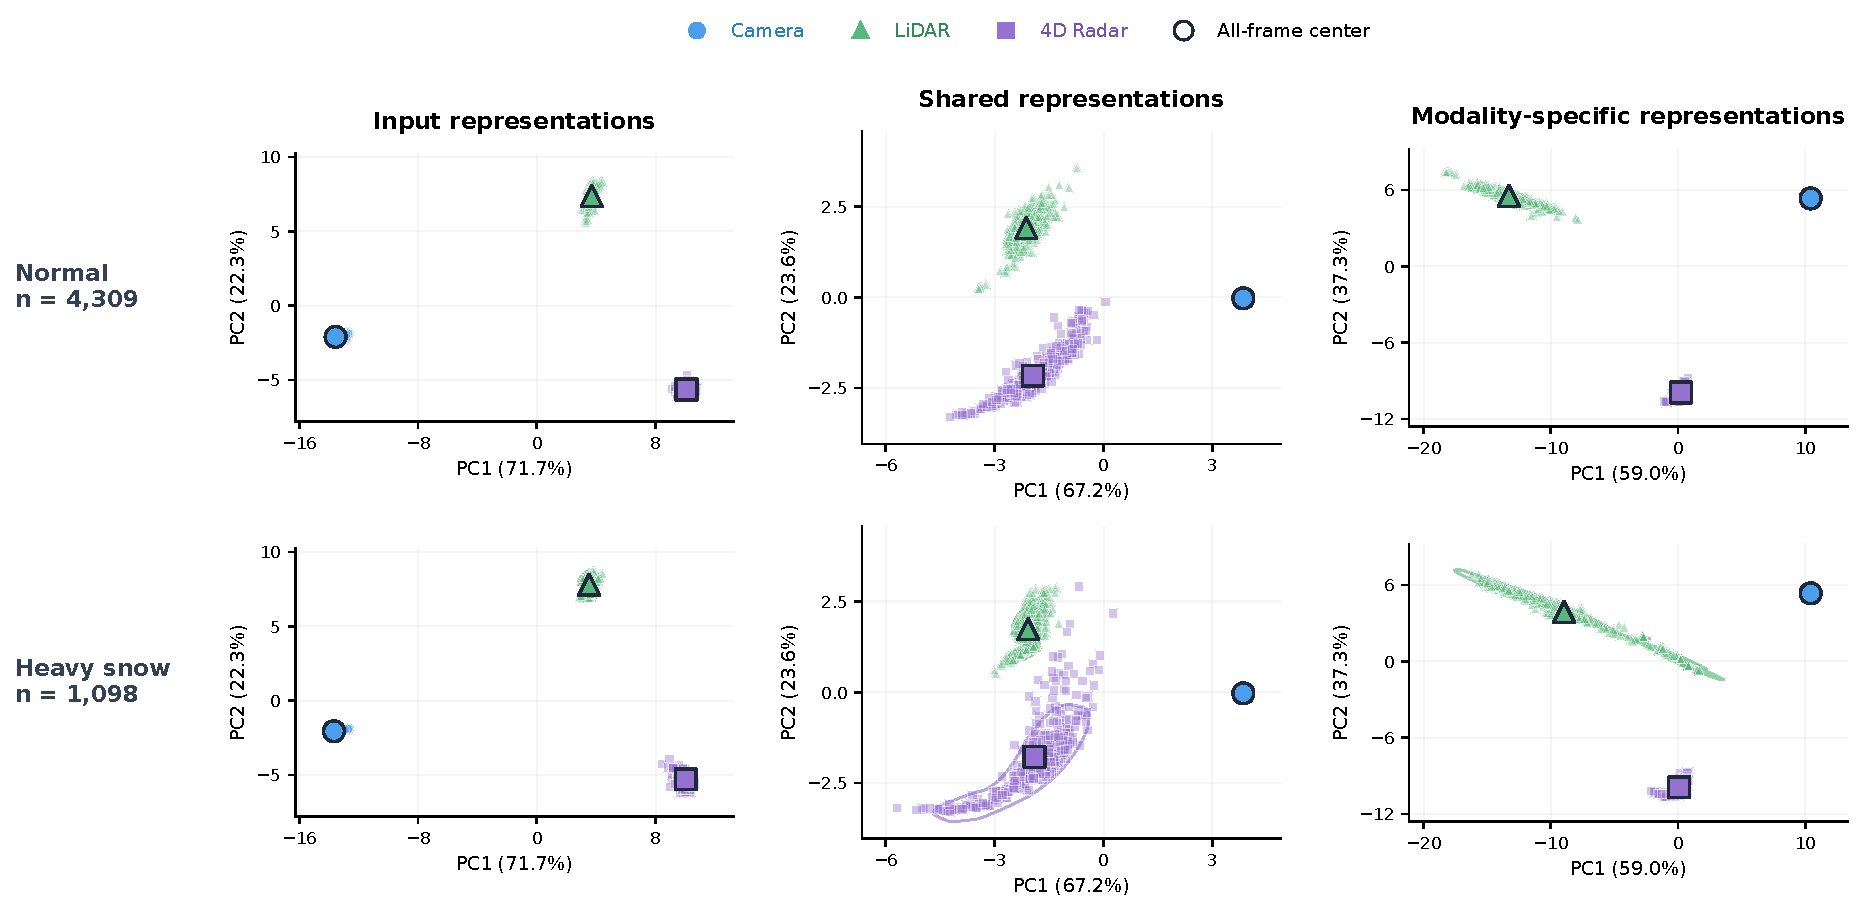
\includegraphics[width=\linewidth]{assets/figure3.pdf}
    \caption{PCA visualization of input, shared, and modality-specific representations on K-Radar v1 under normal and heavy-snow conditions. Each small marker represents the 256-dimensional feature vector averaged over all GT-defined foreground patches of one frame and one modality, projected onto two principal components. Blue circles, green triangles, and purple squares denote camera, LiDAR, and 4D radar, respectively. We display the same 400 randomly sampled frames per weather condition across all columns and modalities. Large outlined markers and density contours are computed using all frames of the corresponding weather group ($n=4{,}309$ and $1{,}098$); contours enclose approximately 80\% of the estimated density where estimation is non-degenerate. A separate PCA basis is fitted for each representation using the full test set with equal total weights for weather groups and modalities; both weather rows share that basis and axis limits within each column. Axis percentages indicate explained variance. GT is used only to select regions for this analysis.}
    \label{fig:3}
\end{figure}


\begin{figure}[t]
    \centering
    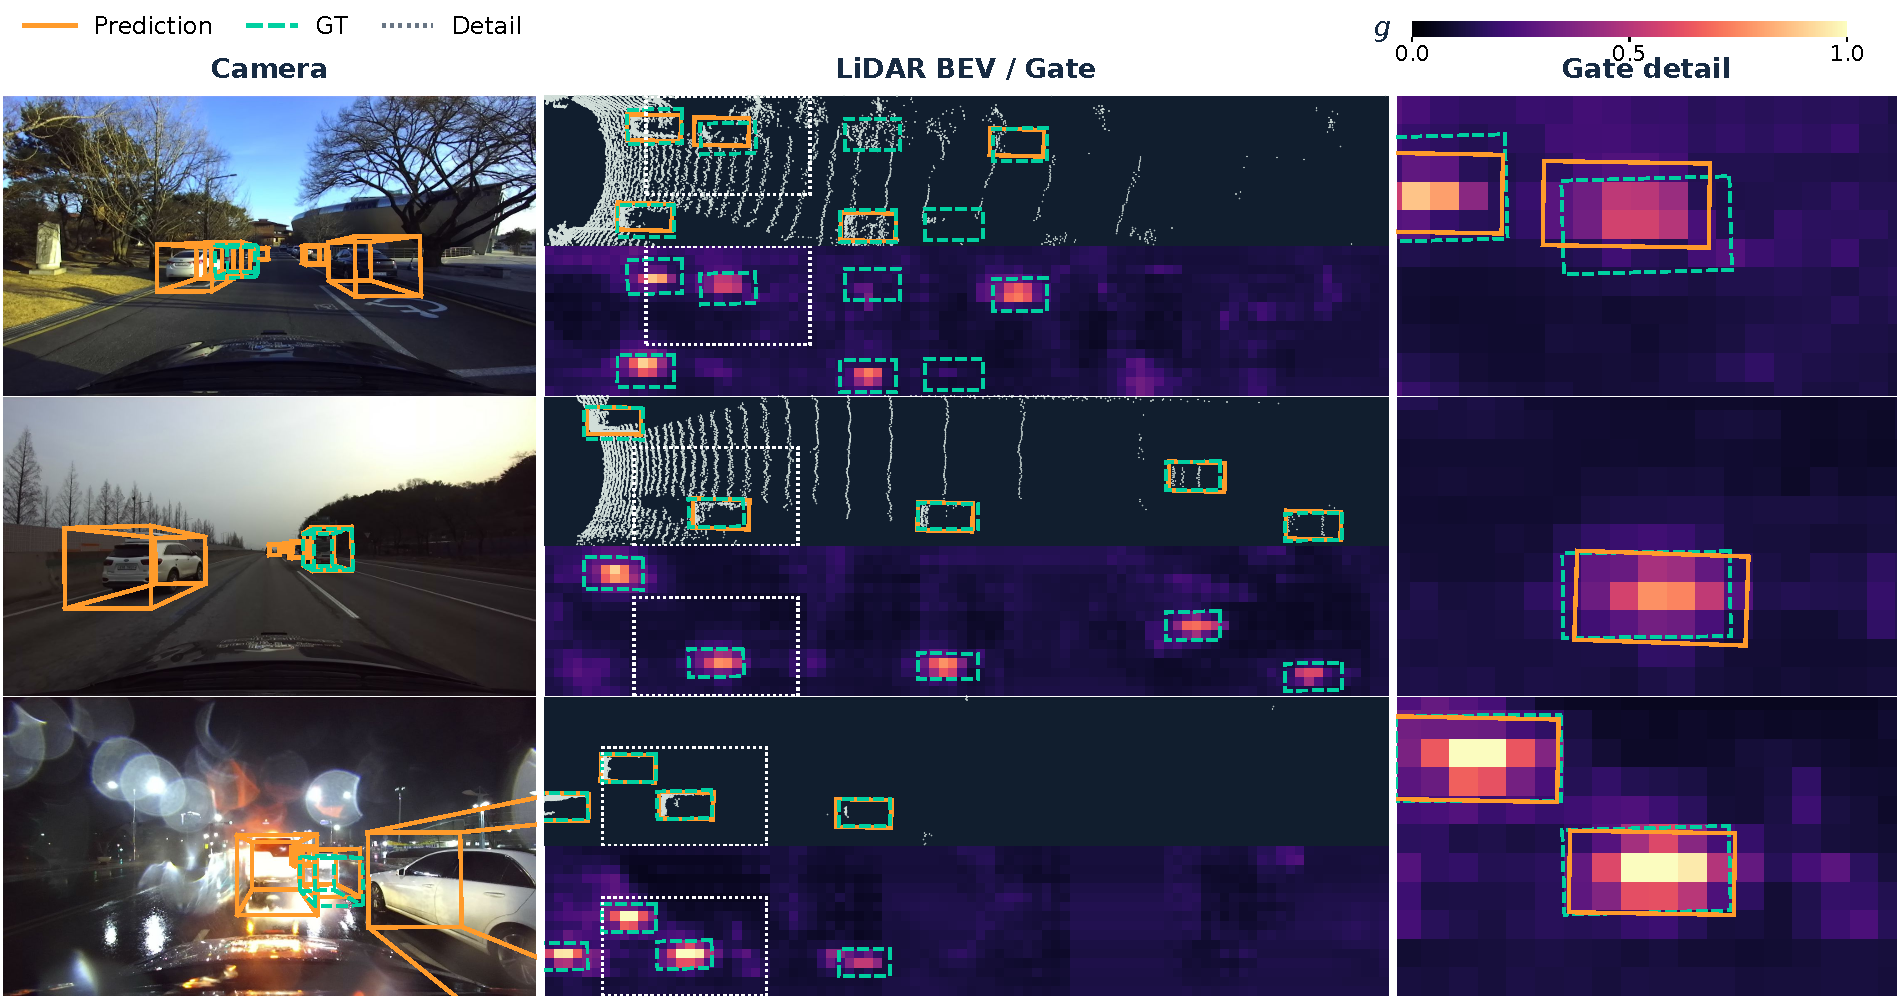
\includegraphics[width=\linewidth]{assets/figure4.pdf}
    \caption{Spatial gating and detection in matched scenes. Each row shows the camera image with ObjDec predictions (left), the full LiDAR BEV and predicted foreground gate (middle, top and bottom), and a magnified gate region (right). Orange solid and green dashed boxes denote predictions with scores above 0.3 and GT references, respectively. Camera panels show the selected target's GT; the BEV and gate panels retain all GT references within their displayed regions. White dotted rectangles mark detail windows. Full BEV views cover $x\in[0,72]$ m and $y\in[-6.4,6.4]$ m; right-hand windows span $14\times8.4$ m, with forward $x$ horizontal and lateral $y$ vertical. All gates use the native 0.8 m grid and a common $[0,1]$ scale without smoothing. Foreground/background gate means are 0.213/0.128, 0.259/0.115, and 0.288/0.118 from top to bottom. Gates are predicted directly from features; GT overlays and region statistics are added after prediction. Gate values modulate fusion and are distinct from detection confidence.}
    \label{fig:4}
\end{figure}


% Paired detections are included only in Appendix E.
